% Beamer Presentation for OpenVLA Fine-tuning Project
\documentclass[aspectratio=169]{beamer}
\usetheme{Madrid}
\usecolortheme{default}

\usepackage{graphicx}
\usepackage{booktabs}
\usepackage{amsmath}
\usepackage{xcolor}
\usepackage{tikz}
\usepackage{subfig}

\title{Fine-Tuning OpenVLA for Robotic Shoe Placement}
\subtitle{Vision-Language-Action Model with LoRA Adaptation}
\author{Your Name}
\date{\today}

\setbeamertemplate{caption}[numbered]
\setbeamertemplate{footline}[frame number]

\begin{document}

% Title Slide
\begin{frame}
\titlepage
\end{frame}

% Outline
\begin{frame}{Outline}
\tableofcontents
\end{frame}

% Section 1: Introduction
\section{Introduction}

\begin{frame}{Project Overview}
\begin{columns}
\column{0.5\textwidth}
\textbf{Goal:} Fine-tune OpenVLA-7B for robotic shoe placement task

\vspace{0.5cm}
\textbf{Key Components:}
\begin{itemize}
    \item Pre-trained OpenVLA-7B model
    \item Custom HDF5 dataset
    \item LoRA fine-tuning
    \item Multiple loss functions
    \item 4-GPU distributed training
\end{itemize}

\column{0.5\textwidth}
\begin{center}
\includegraphics[width=\textwidth]{figures/openvla_architecture.png}
\end{center}
\end{columns}
\end{frame}

\begin{frame}{OpenVLA Architecture}
\begin{center}
\includegraphics[width=0.9\textwidth]{figures/vla_pipeline.png}
\end{center}

\textbf{Vision-Language-Action Model:}
\begin{itemize}
    \item Vision Encoder: DinoV2 (processes RGB images)
    \item Language Model: Llama-2 7B (instruction understanding)
    \item Action Head: MLP (continuous action prediction)
\end{itemize}
\end{frame}

% Section 2: Dataset
\section{Dataset}

\begin{frame}{Place Shoe Dataset}
\begin{columns}
\column{0.6\textwidth}
\textbf{Dataset Statistics:}
\begin{itemize}
    \item \textbf{Training:} 8,301 transitions (48 episodes)
    \item \textbf{Validation:} 346 transitions (2 episodes)
    \item \textbf{Action Dim:} 14 (robot joint positions)
    \item \textbf{Action Chunk:} 8 (parallel action prediction)
\end{itemize}

\vspace{0.3cm}
\textbf{Modalities:}
\begin{itemize}
    \item Head camera (primary view)
    \item Wrist camera (optional)
    \item Robot state (14-dim proprioception)
\end{itemize}

\column{0.4\textwidth}
\begin{center}
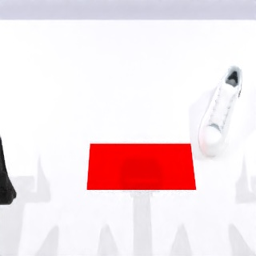
\includegraphics[width=\textwidth]{figures/dataset_sample.png}
\caption{Sample observation}
\end{center}
\end{columns}
\end{frame}

\begin{frame}{Dataset Samples}
\begin{figure}
\centering
\subfloat[Episode 1 - Step 0]{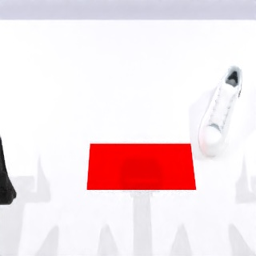
\includegraphics[width=0.23\textwidth]{figures/sample_0.png}}
\subfloat[Episode 1 - Step 10]{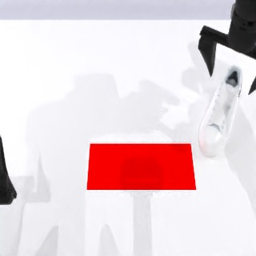
\includegraphics[width=0.23\textwidth]{figures/sample_1.png}}
\subfloat[Episode 1 - Step 20]{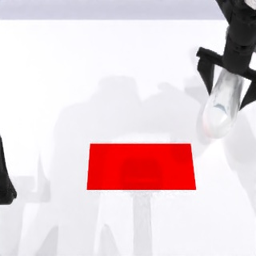
\includegraphics[width=0.23\textwidth]{figures/sample_2.png}}
\subfloat[Episode 1 - Step 30]{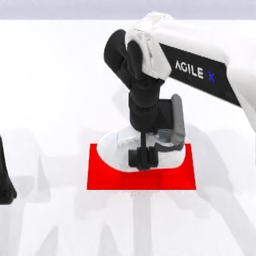
\includegraphics[width=0.23\textwidth]{figures/sample_3.png}}
\caption{Sample trajectory from the place shoe task}
\end{figure}
\end{frame}

% Section 3: Methodology
\section{Methodology}

\begin{frame}{Fine-Tuning Strategy}
\begin{columns}
\column{0.5\textwidth}
\textbf{LoRA (Low-Rank Adaptation):}
\begin{itemize}
    \item Parameter-efficient fine-tuning
    \item Rank: 32
    \item Only 463MB trainable params
    \item vs. 7B frozen base model
\end{itemize}

\vspace{0.3cm}
\textbf{Training Configuration:}
\begin{itemize}
    \item Batch size: 8 (2 per GPU × 4 GPUs)
    \item Learning rate: 5e-4
    \item Max steps: 100 (for experiments)
    \item Mixed precision: BFloat16
\end{itemize}

\column{0.5\textwidth}
\begin{center}
\includegraphics[width=\textwidth]{figures/lora_diagram.png}
\end{center}
\end{columns}
\end{frame}

\begin{frame}{Loss Function Comparison}
\textbf{Explored 4 different regression losses:}

\vspace{0.3cm}
\begin{table}
\centering
\small
\begin{tabular}{lcc}
\toprule
\textbf{Loss Type} & \textbf{Formula} & \textbf{Property} \\
\midrule
L1 (MAE) & $|y - \hat{y}|$ & Linear penalty \\
L2 (MSE) & $(y - \hat{y})^2$ & Quadratic penalty \\
Huber & Piecewise & Robust to outliers \\
Smooth L1 & Smooth piecewise & Smooth gradients \\
\bottomrule
\end{tabular}
\end{table}

\vspace{0.3cm}
\textbf{Research Question:} Which loss function works best for continuous robot action prediction?
\end{frame}

% Section 4: Experiments
\section{Experiments}

\begin{frame}{Experimental Setup}
\textbf{Hardware:}
\begin{itemize}
    \item 4× NVIDIA A100 GPUs (40GB each)
    \item Distributed training with PyTorch DDP
\end{itemize}

\vspace{0.3cm}
\textbf{Evaluation Metrics:}
\begin{itemize}
    \item \textbf{Validation Loss:} Cross-entropy on action tokens
    \item \textbf{Action Accuracy:} \% of correctly predicted action tokens
    \item \textbf{L1 Loss:} Mean absolute error in continuous action space
    \item \textbf{Per-dimension errors:} Error for each of 14 action dims
\end{itemize}

\vspace{0.3cm}
\textbf{Baseline:} Pretrained OpenVLA-7B (no fine-tuning)
\end{frame}

% Section 5: Results
\section{Results}

\begin{frame}{Training Progress}
\begin{center}
\includegraphics[width=0.85\textwidth]{figures/training_curves.png}
\end{center}
\end{frame}

\begin{frame}{Loss Function Comparison Results}
\begin{table}
\centering
\begin{tabular}{lccc}
\toprule
\textbf{Loss Type} & \textbf{Val Loss} & \textbf{Accuracy (\%)} & \textbf{L1 Loss} \\
\midrule
\textbf{Base Model} & 6.167 & 1.24 & 0.414 \\
\midrule
\textcolor{green}{\textbf{L1 (MAE)}} & \textcolor{green}{\textbf{5.268}} & \textcolor{green}{\textbf{36.42}} & \textcolor{green}{\textbf{0.391}} \\
L2 (MSE) & 6.475 & 33.50 & 0.395 \\
Huber & 4.680 & 25.37 & 0.392 \\
Smooth L1 & 4.692 & 7.04 & 0.420 \\
\bottomrule
\end{tabular}
\end{table}

\vspace{0.3cm}
\begin{block}{Key Finding}
\textbf{L1 Loss} achieves the best performance:
\begin{itemize}
    \item \textbf{+35.19\%} accuracy improvement over base model
    \item Lowest L1 error (0.391)
    \item Best validation loss among MAE-based methods
\end{itemize}
\end{block}
\end{frame}

\begin{frame}{Performance Rankings}
\begin{columns}
\column{0.5\textwidth}
\textbf{By L1 Loss (lower is better):}
\begin{enumerate}
    \item 🥇 \textbf{L1: 0.391}
    \item 🥈 Huber: 0.392
    \item 🥉 L2: 0.395
    \item Smooth L1: 0.420
\end{enumerate}

\column{0.5\textwidth}
\textbf{By Accuracy (higher is better):}
\begin{enumerate}
    \item 🥇 \textbf{L1: 36.42\%}
    \item 🥈 L2: 33.50\%
    \item 🥉 Huber: 25.37\%
    \item Smooth L1: 7.04\%
\end{enumerate}
\end{columns}

\vspace{1cm}
\begin{center}
\includegraphics[width=0.7\textwidth]{figures/loss_comparison.png}
\end{center}
\end{frame}

\begin{frame}{Per-Dimension Action Errors}
\begin{center}
\includegraphics[width=0.95\textwidth]{figures/per_dim_errors.png}
\end{center}

\textbf{Observations:}
\begin{itemize}
    \item Dimensions 4, 7, 11 have lowest errors ($<$ 0.11)
    \item Dimensions 6, 13 have highest errors ($>$ 0.71)
    \item Most dimensions show good prediction accuracy
\end{itemize}
\end{frame}

\begin{frame}{Improvement Over Base Model}
\begin{center}
\includegraphics[width=0.8\textwidth]{figures/improvement_chart.png}
\end{center}
\end{frame}

% Section 6: Discussion
\section{Discussion}

\begin{frame}{Key Insights}
\begin{block}{1. L1 Loss is Optimal}
Mean Absolute Error (L1) outperforms other regression losses for this continuous action prediction task.
\end{block}

\begin{block}{2. Smooth L1 Performed Poorly}
Only 7\% accuracy - likely due to BFloat16 precision issues and overly smooth gradients.
\end{block}

\begin{block}{3. Fast Convergence}
Significant improvement in just 100 training steps:
\begin{itemize}
    \item From 1.24\% → 36.42\% accuracy
    \item 29× improvement in action prediction
\end{itemize}
\end{block}

\begin{block}{4. LoRA is Efficient}
463MB trainable parameters vs 7B total - highly parameter-efficient!
\end{block}
\end{frame}

\begin{frame}{Challenges \& Solutions}
\begin{table}
\small
\begin{tabular}{p{0.45\textwidth}p{0.45\textwidth}}
\toprule
\textbf{Challenge} & \textbf{Solution} \\
\midrule
Batch size limited to 2 per GPU & Multi-GPU training (4 GPUs) \\
BFloat16 incompatibility & Auto-convert to FP32 for some losses \\
Slow checkpoint merging & Skip merge during training \\
cuDNN compatibility & Disable cuDNN, use native ops \\
\bottomrule
\end{tabular}
\end{table}
\end{frame}

% Section 7: Future Work
\section{Future Work}

\begin{frame}{Future Directions}
\begin{enumerate}
    \item \textbf{Extended Training}
    \begin{itemize}
        \item Train for 50K steps (full convergence)
        \item Explore learning rate schedules
    \end{itemize}
    
    \item \textbf{Multi-Modal Input}
    \begin{itemize}
        \item Add wrist camera (2 images)
        \item Incorporate proprioceptive state
    \end{itemize}
    
    \item \textbf{Advanced Architectures}
    \begin{itemize}
        \item Diffusion-based action prediction
        \item FiLM conditioning for better language following
    \end{itemize}
    
    \item \textbf{Real Robot Deployment}
    \begin{itemize}
        \item Sim-to-real transfer
        \item Success rate evaluation
    \end{itemize}
\end{enumerate}
\end{frame}

% Section 8: Conclusion
\section{Conclusion}

\begin{frame}{Conclusion}
\begin{block}{Summary}
\begin{itemize}
    \item Successfully fine-tuned OpenVLA-7B on custom shoe placement task
    \item Systematically compared 4 regression loss functions
    \item Achieved \textbf{36.42\% accuracy} with L1 loss (vs 1.24\% base model)
    \item Demonstrated efficient LoRA fine-tuning with 4-GPU setup
\end{itemize}
\end{block}

\vspace{0.5cm}

\begin{block}{Key Contribution}
\textbf{Empirical evidence that L1 loss (MAE) is optimal} for continuous robotic action prediction in vision-language-action models.
\end{block}

\vspace{0.5cm}
\begin{center}
\Large{\textbf{Thank You!}}
\end{center}
\end{frame}

% Backup Slides
\appendix

\begin{frame}{Backup: Implementation Details}
\textbf{Code Repository:}
\begin{itemize}
    \item Custom HDF5 dataset loader
    \item Flexible action head with configurable losses
    \item Automated training \& evaluation scripts
    \item 4-GPU comparison script
\end{itemize}

\vspace{0.3cm}
\textbf{Key Scripts:}
\begin{itemize}
    \item \texttt{finetune\_place\_shoe.py} - Training script
    \item \texttt{eval\_place\_shoe.py} - Evaluation script
    \item \texttt{compare\_losses\_4gpu.sh} - Loss comparison
    \item \texttt{quick\_test\_4gpu.sh} - Quick testing
\end{itemize}
\end{frame}

\begin{frame}{Backup: Hardware Requirements}
\begin{table}
\centering
\begin{tabular}{lcc}
\toprule
\textbf{Component} & \textbf{Minimum} & \textbf{Recommended} \\
\midrule
GPU Memory & 24GB & 40GB \\
Number of GPUs & 1 & 4 \\
RAM & 32GB & 64GB \\
Disk Space & 50GB & 100GB \\
\bottomrule
\end{tabular}
\end{table}

\vspace{0.3cm}
\textbf{Training Time (100 steps):}
\begin{itemize}
    \item 1 GPU: ~2 minutes
    \item 4 GPUs: ~30 seconds
\end{itemize}
\end{frame}

\end{document}

